\section{Notation and Basic Definitions}\label{sec:preliminaries}
In this section, we introduce some basic definitions and results that are used throughout this thesis.
We start with some preliminaries on hypergraphs, which are the main objects of study in this thesis.

\subsection{Hypergraphs}\label{subsec:hypergraphs}

\begin{definition}

    For an integer $k \geq 1$ a \emph{$k$-uniform hypergraph} (or \emph{$k$-graph}, for short)
    is a tuple $G = (V, E)$ where $V$ is a finite set
    and $E \subset \binom{V}{k}$.
    We call the elements of $V(G) = V$ its \emph{vertices}
    and those of $E(G) = E$ its \emph{edges}.
    The value $k$ is called the \emph{uniformity} of $G$.
\end{definition}

\begin{remark}
    In the definition above, if we let $k=1$, we get a set of $1$-sets of the vertex set $V$,
    which we can identify with a subset of $V$.
    If we let $k=2$, we recover the usual definition of an undirected graph with no loops.
\end{remark}

The following definition is a generalization of the notion of degree
of a vertex in a graph.

\begin{definition}
    Let $G = (V, E)$ be a $k$-graph and $v \in V$.
    The \emph{degree} $d_G(v)$ of $v$ in $G$
    is the number of edges containing $v$, that is
    \[
        d_G(v) = |\{e \in E \mid v \in e\}|.
    \]
\end{definition}

A useful operation is restricting a k-graph to a subset of its vertices.
This yields a new k-graph, called the \emph{subgraph induced by} the subset, which has the same uniformity.

\begin{definition}

    \label{def:restriction}
    Let $G = (V, E)$ be a $k$-graph and $T \subset V$.
    The \emph{restriction} of $G$ to $T$ is the $k$-graph
    \[
        G[T] = (T, E_T),
    \]
    where
    \[E_T = \{e \in E \mid e \subset T\}.\]
\end{definition}

The following operation also lets us obtain graphs of a
different uniformity from a subset of vertices of a $k$-graph.

\begin{definition} \label{def:link}
    Let $G = (V, E)$ be a $k$-graph.
    Let $1 \leq j \leq k - 1$ be an integer and let
    $T \subset V$ be a set of vertices satisfying $k - j \leq |T|$.
    The \emph{common $j$-link graph} of $T$ is the $j$-graph $\link{G}{T}{j} = (V \setminus T, E')$, where
    \[
        E' = \left\{Y \in \binom{V \setminus T}{j}\middle\vert \, X \cup Y \in E \text{ for all } X \in \binom{T}{k-j}\right\}.
    \]
\end{definition}

Figure~\ref{fig:link} illustrates how to construct
a common $j$-link graph from a $k$-graph $G$ in the case $k=3$ and $j=2$.

\begin{figure}[ht]
    \centering
    % TikZ code generated by Python script for Common Link Graph visualization
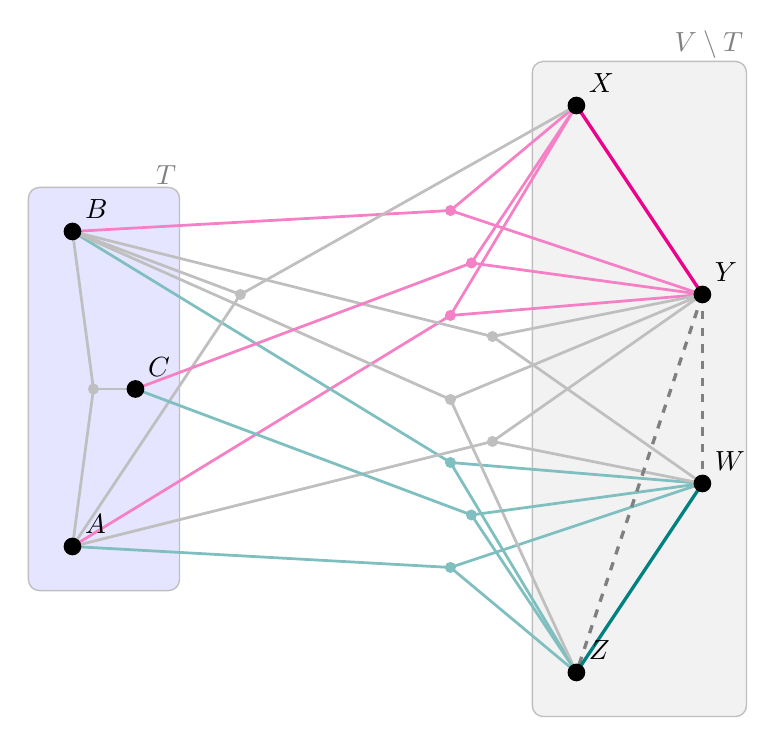
\begin{tikzpicture}[scale=0.8]
% Vertex coordinates
\coordinate (A) at (0.00, 2.00);
\coordinate (B) at (0.00, 7.00);
\coordinate (C) at (1.00, 4.50);
\coordinate (X) at (8.00, 9.00);
\coordinate (Y) at (10.00, 6.00);
\coordinate (Z) at (8.00, 0.00);
\coordinate (W) at (10.00, 3.00);
% Hyperedge root coordinates
\coordinate (R0) at (6.000, 5.667);
\coordinate (R2) at (6.000, 7.333);
\coordinate (R3) at (6.667, 5.333);
\coordinate (R4) at (6.000, 1.667);
\coordinate (R5) at (6.000, 3.333);
\coordinate (R6) at (2.667, 6.000);
\coordinate (R7) at (6.667, 3.667);
\coordinate (R8) at (6.000, 4.333);
\coordinate (R9) at (0.333, 4.500);
\coordinate (R10) at (6.333, 6.500);
\coordinate (R11) at (6.333, 2.500);
% Draw background boxes for T and V \ T
\draw[fill=blue!10, rounded corners, line width=0.5pt, draw=gray!50] (-0.70, 1.30) rectangle (1.70, 7.70);
\node at (1.70, 7.70) [anchor=south east, inner sep=1pt, text=gray] {$T$};
\draw[fill=gray!10, rounded corners, line width=0.5pt, draw=gray!50] (7.30, -0.70) rectangle (10.70, 9.70);
\node at (10.70, 9.70) [anchor=south east, inner sep=1pt, text=gray] {$V \setminus T$};
% Draw original hyperedges (styled by category)
\draw[line width=1.0pt, color=magenta!50!white, solid] (R0) -- (A);
\draw[line width=1.0pt, color=magenta!50!white, solid] (R0) -- (X);
\draw[line width=1.0pt, color=magenta!50!white, solid] (R0) -- (Y);
\fill[magenta!50!white] (R0) circle (2.5pt);
\draw[line width=1.0pt, color=magenta!50!white, solid] (R2) -- (B);
\draw[line width=1.0pt, color=magenta!50!white, solid] (R2) -- (X);
\draw[line width=1.0pt, color=magenta!50!white, solid] (R2) -- (Y);
\fill[magenta!50!white] (R2) circle (2.5pt);
\draw[line width=1.0pt, color=gray!50!white, solid] (R3) -- (B);
\draw[line width=1.0pt, color=gray!50!white, solid] (R3) -- (Y);
\draw[line width=1.0pt, color=gray!50!white, solid] (R3) -- (W);
\fill[gray!50!white] (R3) circle (2.5pt);
\draw[line width=1.0pt, color=teal!50!white, solid] (R4) -- (A);
\draw[line width=1.0pt, color=teal!50!white, solid] (R4) -- (Z);
\draw[line width=1.0pt, color=teal!50!white, solid] (R4) -- (W);
\fill[teal!50!white] (R4) circle (2.5pt);
\draw[line width=1.0pt, color=teal!50!white, solid] (R5) -- (B);
\draw[line width=1.0pt, color=teal!50!white, solid] (R5) -- (Z);
\draw[line width=1.0pt, color=teal!50!white, solid] (R5) -- (W);
\fill[teal!50!white] (R5) circle (2.5pt);
\draw[line width=1.0pt, color=gray!50!white, solid] (R6) -- (A);
\draw[line width=1.0pt, color=gray!50!white, solid] (R6) -- (B);
\draw[line width=1.0pt, color=gray!50!white, solid] (R6) -- (X);
\fill[gray!50!white] (R6) circle (2.5pt);
\draw[line width=1.0pt, color=gray!50!white, solid] (R7) -- (A);
\draw[line width=1.0pt, color=gray!50!white, solid] (R7) -- (Y);
\draw[line width=1.0pt, color=gray!50!white, solid] (R7) -- (W);
\fill[gray!50!white] (R7) circle (2.5pt);
\draw[line width=1.0pt, color=gray!50!white, solid] (R8) -- (B);
\draw[line width=1.0pt, color=gray!50!white, solid] (R8) -- (Y);
\draw[line width=1.0pt, color=gray!50!white, solid] (R8) -- (Z);
\fill[gray!50!white] (R8) circle (2.5pt);
\draw[line width=1.0pt, color=gray!50!white, solid] (R9) -- (A);
\draw[line width=1.0pt, color=gray!50!white, solid] (R9) -- (B);
\draw[line width=1.0pt, color=gray!50!white, solid] (R9) -- (C);
\fill[gray!50!white] (R9) circle (2.5pt);
\draw[line width=1.0pt, color=magenta!50!white, solid] (R10) -- (C);
\draw[line width=1.0pt, color=magenta!50!white, solid] (R10) -- (X);
\draw[line width=1.0pt, color=magenta!50!white, solid] (R10) -- (Y);
\fill[magenta!50!white] (R10) circle (2.5pt);
\draw[line width=1.0pt, color=teal!50!white, solid] (R11) -- (C);
\draw[line width=1.0pt, color=teal!50!white, solid] (R11) -- (Z);
\draw[line width=1.0pt, color=teal!50!white, solid] (R11) -- (W);
\fill[teal!50!white] (R11) circle (2.5pt);
% Draw 'almost' link edges (faintly, dotted)
\draw[color=gray, very thick, dashed] (Y) -- (Z);
\draw[color=gray, very thick, dashed] (Y) -- (W);
% Edges of the common 2-link graph of T (brightly colored)
\draw[very thick, color=magenta] (X) -- (Y);
\draw[very thick, color=teal] (Z) -- (W);
% Draw vertices (foreground layer)
\fill[black] (A) circle (4.0pt);
\node[above right=1pt, color=black] at (A) {$A$};
\fill[black] (B) circle (4.0pt);
\node[above right=1pt, color=black] at (B) {$B$};
\fill[black] (C) circle (4.0pt);
\node[above right=1pt, color=black] at (C) {$C$};
\fill[black] (X) circle (4.0pt);
\node[above right=1pt, color=black] at (X) {$X$};
\fill[black] (Y) circle (4.0pt);
\node[above right=1pt, color=black] at (Y) {$Y$};
\fill[black] (Z) circle (4.0pt);
\node[above right=1pt, color=black] at (Z) {$Z$};
\fill[black] (W) circle (4.0pt);
\node[above right=1pt, color=black] at (W) {$W$};
\end{tikzpicture}
    \caption{A $3$-graph $G$ and the common $2$-link graph $\link{G}{T}{2}$ of the set $T = \{A, B, C\}$.
        Vertices are represented as black dots, and $3$-edges of $G$ are represented as colored or gray small dots,
        connected by a line to the vertices they contain.
        Colored dots correspond to $3$-edges with exactly
        $k - j = 3 - 2 = 1$ vertices in $T$, which are the only ones that can contribute to the common $2$-link graph.
        Edges in the common $2$-link graph are represented as solid lines connecting the corresponding vertices,
        in the same color that the $3$-edges they come from.
        Dashed lines correspond to edge pairs
        in $V \setminus T$ that have some of the required $3$-edges in $G$, but not all of them.
        The resulting link graph has vertex set $\{X, Y, Z, W\}$ and edge set
        $\{\{X, Y\}, \{W, Z\}\}$.
    }
    \label{fig:link}
\end{figure}

Next, we introduce $k$-graph homomorphisms, embeddings and isomorphisms, which allow us
to relate $k$-graphs of the same uniformity to each other.

\begin{definition} \label{def:embedding}
    Let $G = (V, E)$ and $H = (W, F)$ be $k$-graphs and let $f: V \to W$ be a map
    between their vertex sets.
    If $A \subset E$ is a set of edges in $G$, we denote
    \[
        f(A) = \{f(e) \mid e \in A\} = \{\{f(v) \mid v \in e\} \mid e \in A\}.
    \]
    Then, $f$ is a \emph{homomorphism} from $G$ to $H$ if
    \begin{equation}
        \label{eq:homomorphism}
        f(E) \subset E(H[f(V)]).
    \end{equation}
    If such a homomorphism exists
    and is injective, we say that $f$ is an \emph{embedding} of $G$ on $H$
    and that $H$ \emph{contains} $G$ as a subgraph.
    We write $G \subset H$.
    Otherwise, we say that $H$ is $G$-\emph{free}.

    If $f$ is an embedding of $G$ in $H$ and
    \begin{equation}
        \label{eq:induced_embedding}
        f(E) = E(H[f(V)]),
    \end{equation}
    we say that $f$ is an \emph{induced} embedding
    and that $H$ contains $G$ as an \emph{induced} subgraph.
    We write $G \subset_{\text{ind}} H$.
    If, in addition, $f$ is a bijection, we say that $f$ is an \emph{isomorphism}
    and that $G$ is \emph{isomorphic} to $H$.
    We write $G \cong H$.
\end{definition}

\begin{remark}
    Condition~\eqref{eq:homomorphism} of definition~\ref{def:embedding}
    implies that $f$ is injective
    when restricted to each edge in $E$, because $G$ and $H$ have the same uniformity.
    However, it does not necessarily imply that $f$ is injective on all of $V$.
\end{remark}

It can be checked that isomorphism of $k$-graphs is an equivalence relation.
Furthermore, it is compatible with the subgraph ($\subset$) and induced subgraph
($\subset_{\text{ind}}$) relations, which are preorders.
This allows us to discuss whether a graph $G$ is an (induced) subgraph of another graph $H$,
\emph{ up to isomorphism} in both the \emph{guest} graph $G$ and the \emph{host} graph $H$.
For more details, see Appendix~\ref{apx:embeddings-properties}.

So far, we have not seen any concrete examples of $k$-graphs or their isomorphism classes.
We now introduce an important family of them.

\begin{definition} \label{def:complete}
    A $k$-graph $G = (V, E)$ is \emph{complete} if $E = \binom{V}{k}$.
    We denote $G = \completesuperindex{k}{V}$
\end{definition}

If $K$ and $K'$ are complete $k$-graphs with the same number of vertices $r$,
any bijection $f: V(K) \to V(K')$ is clearly an isomorphism between $K$ and $K'$.
This allows us to talk, up to isomorphism, about \emph{the} complete $k$-graph on $r$ vertices $\completesuperindex{k}{r}$.
For example, in Figure~\ref{fig:complete_kgraph} we show the complete graph $\completesuperindex{3}{4}$.

\begin{figure}[htbp]
    \centering
    % TikZ code for K_4^(3) using predefined edge colors
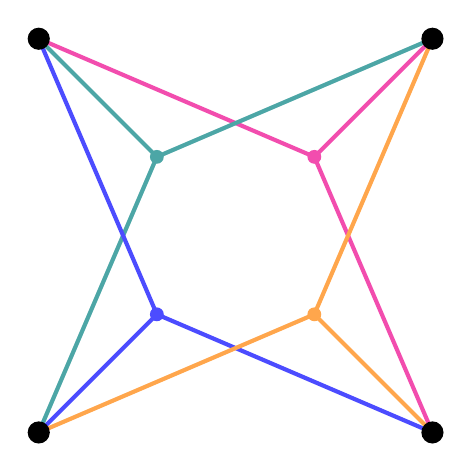
\begin{tikzpicture}[scale=1]
\coordinate (V1) at (0, 5);
\coordinate (V2) at (5, 5);
\coordinate (V3) at (5, 0);
\coordinate (V4) at (0, 0);
\coordinate (R0) at (3.500, 3.500);
\draw[line width=1.5pt, color=magenta!70!white] (R0) -- (V1);
\draw[line width=1.5pt, color=magenta!70!white] (R0) -- (V2);
\draw[line width=1.5pt, color=magenta!70!white] (R0) -- (V3);
\fill[color=magenta!70!white] (R0) circle (2.5pt);
\coordinate (R1) at (1.500, 3.500);
\draw[line width=1.5pt, color=teal!70!white] (R1) -- (V1);
\draw[line width=1.5pt, color=teal!70!white] (R1) -- (V2);
\draw[line width=1.5pt, color=teal!70!white] (R1) -- (V4);
\fill[color=teal!70!white] (R1) circle (2.5pt);
\coordinate (R2) at (1.500, 1.500);
\draw[line width=1.5pt, color=blue!70!white] (R2) -- (V1);
\draw[line width=1.5pt, color=blue!70!white] (R2) -- (V3);
\draw[line width=1.5pt, color=blue!70!white] (R2) -- (V4);
\fill[color=blue!70!white] (R2) circle (2.5pt);
\coordinate (R3) at (3.500, 1.500);
\draw[line width=1.5pt, color=orange!70!white] (R3) -- (V2);
\draw[line width=1.5pt, color=orange!70!white] (R3) -- (V3);
\draw[line width=1.5pt, color=orange!70!white] (R3) -- (V4);
\fill[color=orange!70!white] (R3) circle (2.5pt);
\fill[black] (V1) circle (4.0pt);
\fill[black] (V2) circle (4.0pt);
\fill[black] (V3) circle (4.0pt);
\fill[black] (V4) circle (4.0pt);
\end{tikzpicture}
    \caption{A complete $3$-graph on $4$ vertices.}
    \label{fig:complete_kgraph}
\end{figure}

\begin{remark}
    A $k$-graph $H = (V, E)$ contains $G = \completesuperindex{k}{r}$ as a subgraph if and only if,
    for some subset $T \subset V$ of size $r$, (namely, the image of an embedding of $G$)
    $H[T] \subset H$ is complete.
    Such an embedding is always induced, as it is given by the identity map on $T$.
\end{remark}

\subsection{Partite Hypergraphs}\label{subsec:partite}

One way to impose structure on a $k$-graph is to require that it is \emph{partite}.

\begin{definition} \label{def:partite} % TODO why does richard say you do not recover the chromatic number?
    for an integer $r \geq k$, a $k$-graph $G = (V, E)$ is \emph{$r$-partite}
    (or $(r, 1)$-\emph{colorable})
    if there exists a partition $V = V_1 \cup \dots \cup V_r$
    such that every edge $e \in E$ intersects every part $V_i$ in at most one vertex.
    We may write $G = (V_1, \dots, V_r; E)$ and say that
    $G$ is a partite $k$-graph on $V_1, \dots, V_r$.
    If $r$ is the minimum integer such that $G$ is $r$-partite,
    we say that $r = \chi_{1}(G)$ is the \emph{partiteness} of $G$.
\end{definition}

The above definition is a special case of the family of chromatic numbers of hypergraphs $\chi_{\gamma}(G)$,
where the condition is that an edge of the hypergraph can intersect each part in at most
$\gamma$ vertices ~\cite{krivelevich1998chromatic}.
If we set $\gamma = k - 1$, we recover the usual notion of chromatic number $\chi(G)$,
in which we impose that edges are not fully contained in any part.
In general, this is much weaker, but the two notions are the same when $k = 2$.

\begin{remark}
    These chromatic numbers are monotone non-decreasing with respect to the subgraph relation.
    Indeed, if $f: G \to H$ is an embedding of $k$-graphs,
    and $H$ is $(r, \gamma)$-partite with parts $V_1, \dots, V_r$,
    then $G$ is $(r, \gamma)$-partite with parts $f^{-1}(V_1), \dots, f^{-1}(V_r)$.
    This is because $f$ is injective, so it preserves the number of vertices in each part for every edge.
    This in turn means that $\chi_{\gamma}(G) \leq \chi_{\gamma}(H)$.
\end{remark}

If $G = (V_1, \dots, V_k; E)$ is a $k$-partite $k$-graph,
every edge intersects every part in exactly one vertex.
This means that we can identify the edges with a subset of $ V_1 \times \dots \times V_k$.
If it is clear from context, we may slightly abuse notation when talking about ordered and
unordered sets of vertices, as in the definition below.


\begin{definition} \label{def:complete_kpartite}
    A $k$-partite $k$-graph $G = (V_1, \dots, V_k; E)$ is \emph{complete}
    if $E = V_1 \times \dots \times V_k$.
    That is, if all $(v_1, \dots, v_k) \in V_1 \times \dots \times V_k$
    satisfy $\{v_1, \dots, v_k\} \in E$.
    We denote $G = \compdots{V_1}{V_k}$.
\end{definition}

In some cases, it is useful to generalize this notation to partite $k$-graphs
where the number of parts is different from $k$.

\begin{definition}
    Let $r \geq k \geq 1$.
    An $r$-partite $k$-graph $G = (V_1, \dots, V_r; E)$ is \emph{complete} if
    \[
        E = \bigcup_{\left\{i_1, \dots, i_k \right\} \in \binom{[r]}{k}} V_{i_1} \times \dots \times V_{i_k}.
    \]
    We denote $G = \compdotssuperindex{k}{V_1}{V_r}$.

\end{definition}

If $V_1, \dots, V_r$ and $W_1, \dots, W_r$ are disjoint sets
and $|V_i| = |W_i| = a_i$ for all $i$, then
\[
    \compdotssuperindex{k}{V_1}{V_r} \cong \compdotssuperindex{k}{W_1}{W_r}.
\]
An isomorphism is given by any bijection $f: V \to W$ (where $V=\bigcup_i V_i, W=\bigcup_i W_i$)
such that $f(V_i) = W_i$ for all $i$.
This allows us to talk, up to isomorphism, about \emph{the} complete $r$-partite $k$-graph
with part sizes $a_1, \dots, a_r$, which we denote by
\[
    \compdotssuperindex{k}{a_1}{a_r},
\]
or, in the $k$-partite case, by
\[
    K(a_1, \dots, a_k) = K^{(k)}(a_1, \dots, a_k).
\]

\begin{figure}[htbp]
    \centering
    % TikZ code for K^(3)(2, 2, 2) using predefined edge colors
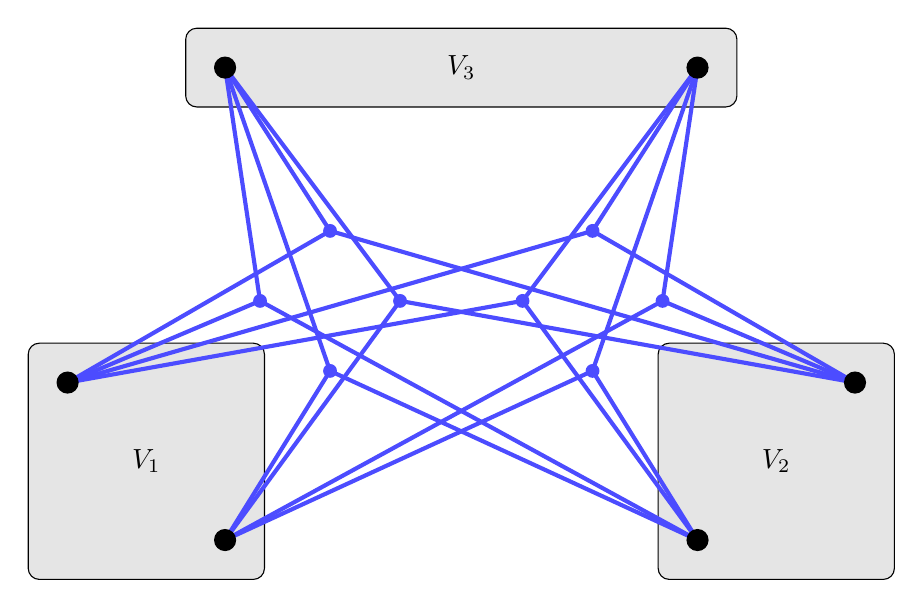
\begin{tikzpicture}[scale=1]
\draw[fill=gray!20, rounded corners] (-0.50, -0.50) rectangle (2.50, 2.50);
\node at (1.00, 1.00) [align=center] {$V_1$};
\draw[fill=gray!20, rounded corners] (7.50, -0.50) rectangle (10.50, 2.50);
\node at (9.00, 1.00) [align=center] {$V_2$};
\draw[fill=gray!20, rounded corners] (1.50, 5.50) rectangle (8.50, 6.50);
\node at (5.00, 6.00) [align=center] {$V_3$};
\coordinate (A1) at (2, 0);
\coordinate (A2) at (0, 2);
\coordinate (B1) at (8, 0);
\coordinate (B2) at (10, 2);
\coordinate (C1) at (2, 6);
\coordinate (C2) at (8, 6);
\coordinate (R0) at (3.333, 2.148);
\draw[line width=1.5pt, color=blue!70!white] (R0) -- (A1);
\draw[line width=1.5pt, color=blue!70!white] (R0) -- (B1);
\draw[line width=1.5pt, color=blue!70!white] (R0) -- (C1);
\fill[color=blue!70!white] (R0) circle (2.5pt);
\coordinate (R1) at (6.667, 2.148);
\draw[line width=1.5pt, color=blue!70!white] (R1) -- (A1);
\draw[line width=1.5pt, color=blue!70!white] (R1) -- (B1);
\draw[line width=1.5pt, color=blue!70!white] (R1) -- (C2);
\fill[color=blue!70!white] (R1) circle (2.5pt);
\coordinate (R2) at (4.222, 3.037);
\draw[line width=1.5pt, color=blue!70!white] (R2) -- (A1);
\draw[line width=1.5pt, color=blue!70!white] (R2) -- (B2);
\draw[line width=1.5pt, color=blue!70!white] (R2) -- (C1);
\fill[color=blue!70!white] (R2) circle (2.5pt);
\coordinate (R3) at (7.556, 3.037);
\draw[line width=1.5pt, color=blue!70!white] (R3) -- (A1);
\draw[line width=1.5pt, color=blue!70!white] (R3) -- (B2);
\draw[line width=1.5pt, color=blue!70!white] (R3) -- (C2);
\fill[color=blue!70!white] (R3) circle (2.5pt);
\coordinate (R4) at (2.444, 3.037);
\draw[line width=1.5pt, color=blue!70!white] (R4) -- (A2);
\draw[line width=1.5pt, color=blue!70!white] (R4) -- (B1);
\draw[line width=1.5pt, color=blue!70!white] (R4) -- (C1);
\fill[color=blue!70!white] (R4) circle (2.5pt);
\coordinate (R5) at (5.778, 3.037);
\draw[line width=1.5pt, color=blue!70!white] (R5) -- (A2);
\draw[line width=1.5pt, color=blue!70!white] (R5) -- (B1);
\draw[line width=1.5pt, color=blue!70!white] (R5) -- (C2);
\fill[color=blue!70!white] (R5) circle (2.5pt);
\coordinate (R6) at (3.333, 3.926);
\draw[line width=1.5pt, color=blue!70!white] (R6) -- (A2);
\draw[line width=1.5pt, color=blue!70!white] (R6) -- (B2);
\draw[line width=1.5pt, color=blue!70!white] (R6) -- (C1);
\fill[color=blue!70!white] (R6) circle (2.5pt);
\coordinate (R7) at (6.667, 3.926);
\draw[line width=1.5pt, color=blue!70!white] (R7) -- (A2);
\draw[line width=1.5pt, color=blue!70!white] (R7) -- (B2);
\draw[line width=1.5pt, color=blue!70!white] (R7) -- (C2);
\fill[color=blue!70!white] (R7) circle (2.5pt);
\fill[black] (A1) circle (4.0pt);
\fill[black] (A2) circle (4.0pt);
\fill[black] (B1) circle (4.0pt);
\fill[black] (B2) circle (4.0pt);
\fill[black] (C1) circle (4.0pt);
\fill[black] (C2) circle (4.0pt);
\end{tikzpicture}
    \caption{The complete 3-partite 3-graph $K(2, 2, 2)$, with parts $V_1, V_2, V_3$.}
    \label{fig:222}
\end{figure}

\begin{figure}[htbp]
    \centering
    % TikZ code for K^(2)(2, 2, 2) using predefined edge colors
\pgfdeclarelayer{background}
\pgfdeclarelayer{main}
\pgfsetlayers{background,main}
\begin{tikzpicture}[scale=0.8]
\begin{pgfonlayer}{background}
  \draw[fill=gray!20, rounded corners] (0.30, 0.30) rectangle (1.70, 3.70);
\end{pgfonlayer}
\node at (1.00, 2.00) [align=center] {$V_1$};
\begin{pgfonlayer}{background}
  \draw[fill=gray!20, rounded corners] (8.30, 0.30) rectangle (9.70, 3.70);
\end{pgfonlayer}
\node at (9.00, 2.00) [align=center] {$V_2$};
\begin{pgfonlayer}{background}
  \draw[fill=gray!20, rounded corners] (4.30, 5.30) rectangle (5.70, 8.70);
\end{pgfonlayer}
\node at (5.00, 7.00) [align=center] {$V_3$};
\coordinate (A1) at (1, 1);
\coordinate (A2) at (1, 3);
\coordinate (B1) at (9, 1);
\coordinate (B2) at (9, 3);
\coordinate (C1) at (5, 6);
\coordinate (C2) at (5, 8);
\draw[line width=1.5pt, color=magenta!60!white] (A1) -- (B1);
\draw[line width=1.5pt, color=magenta!60!white] (A1) -- (B2);
\draw[line width=1.5pt, color=magenta!60!white] (A2) -- (B1);
\draw[line width=1.5pt, color=magenta!60!white] (A2) -- (B2);
\draw[line width=1.5pt, color=teal!60!white] (A1) -- (C1);
\draw[line width=1.5pt, color=teal!60!white] (A1) -- (C2);
\draw[line width=1.5pt, color=teal!60!white] (A2) -- (C1);
\draw[line width=1.5pt, color=teal!60!white] (A2) -- (C2);
\draw[line width=1.5pt, color=orange!60!white] (B1) -- (C1);
\draw[line width=1.5pt, color=orange!60!white] (B1) -- (C2);
\draw[line width=1.5pt, color=orange!60!white] (B2) -- (C1);
\draw[line width=1.5pt, color=orange!60!white] (B2) -- (C2);
\begin{pgfonlayer}{main}
  \fill[black] (A1) circle (4.0pt);
  \fill[black] (A2) circle (4.0pt);
  \fill[black] (B1) circle (4.0pt);
  \fill[black] (B2) circle (4.0pt);
  \fill[black] (C1) circle (4.0pt);
  \fill[black] (C2) circle (4.0pt);
\end{pgfonlayer}
\end{tikzpicture}
    \caption{The complete 3-partite 2-graph $K^{(2)}(2, 2, 2)$, with parts $V_1, V_2, V_3$.}
    \label{fig:k2_222}
\end{figure}

Figure~\ref{fig:222} shows the complete $3$-partite $3$-graph
with $2$ vertices in each part, $K(2, 2, 2) = K^{(3)}(2, 2, 2)$.
In contrast, Figure~\ref{fig:k2_222} shows the complete $3$-partite $2$-graph
$K^{(2)}(2, 2, 2)$.

\subsection{Blowing Up} \label{subsec:blowup}
Another interesting operation we can do with $k$-graphs is the following.

\begin{definition}
    Let $G = (\{v_1, \dots, v_p\}, E)$ be a $k$-graph and let $t$ be a positive integer.
    The $t$-\emph{blowup} $G(t)$ of $G$ is the $p$-partite $k$-graph
    \[
        G(t) = (V_1, \dots, V_p; E')
    \]
    where $|V_i| = t$ and
    \[
        E' = \bigcup_{v_{i_1}, \dots, v_{i_k} \in E} V_{i_1} \times \dots \times V_{i_k}.
    \]
\end{definition}

In essence, we replace each vertex with a set of $t$ vertices, and each edge with a complete $k$-partite $k$-graph
on the corresponding parts.
For example, Figure~\ref{fig:k2_222} displays the $2$-blowup of the triangle graph \completesuperindex{2}{3},
with the edges corresponding to the three original edges of the triangle shown in different colors.
Any complete $p$-partite $k$-graph with equal part sizes can be seen as a blowup of a complete $k$-graph.
In particular, the complete $k$-graph $\compoverset{k}{t}$ (see Figure~\ref{fig:222} for an example)
is often known as a \emph{blowup of an edge}, because it is a $t$-blowup of the
$k$-graph on $k$ vertices with a single edge $\completesuperindex{k}{k}$.
Similarly to the case of complete $k$-graphs and complete $k$-partite $k$-graphs,
the $t$-blowup of a $k$-graph is unique up to isomorphism.

\subsection{Asymptotic Notation}\label{subsec:asymptotic-notation} % Corrected spelling

Throughout this thesis, we will often describe the growth rate of functions whose domain is the set of positive integers $\mathbb{N}$. Unless otherwise stated, the functions we consider map to non-negative real numbers $\mathbb{R}_{\ge 0}$. We now introduce some standard asymptotic notations.

\begin{definition}
    Let $f: \mathbb{N} \to \mathbb{R}_{\ge 0}$ be a function.
    We define $\bigO{f}$ to be the set of functions $g: \mathbb{N} \to \mathbb{R}_{\ge 0}$ such that there exist a constant $C > 0$ and an integer $n_0 \in \mathbb{N}$ for which
    \[
        g(n) \leq C \cdot f(n) \quad \text{for all } n \geq n_0.
    \]
\end{definition}

As a common shorthand, we write $g(n) = \bigO{f(n)}$ to mean $g \in \bigO{f}$.
This notation is also used in arithmetic expressions.
For example, if $h$ is the function $n \mapsto n^2$,
an expression like $e^n + \bigO{n^2}$ denotes the set of functions $\{n \mapsto e^n + k(n) \mid k \in \bigO{h}\}$.

\begin{definition}
    Let $f: \mathbb{N} \to \mathbb{R}_{\ge 0}$ be a function.
    We define $\Omega(f)$ to be the set of functions $g: \mathbb{N} \to \mathbb{R}_{\ge 0}$ such that there exist a constant $c > 0$ and an integer $n_0 \in \mathbb{N}$ for which
    \[
        g(n) \geq c \cdot f(n) \quad \text{for all } n \geq n_0.
    \]
    As shorthand, we write $g(n) = \Omega(f(n))$ for $g \in \Omega(f)$.
\end{definition}

\begin{definition}
    Let $f: \mathbb{N} \to \mathbb{R}_{\ge 0}$ be a function.
    We define $\Theta(f)$ to be the set of functions $g: \mathbb{N} \to \mathbb{R}_{\ge 0}$ such that there exist constants $c_1 > 0, c_2 > 0$ and an integer $n_0 \in \mathbb{N}$ for which
    \[
        c_1 \cdot f(n) \leq g(n) \leq c_2 \cdot f(n) \quad \text{for all } n \geq n_0.
    \]
    Equivalently, $\Theta(f) = \bigO{f} \cap \Omega(f)$, assuming $f, g$ are non-negative.
    As shorthand, we write $g(n) = \Theta(f(n))$ for $g \in \Theta(f)$.
\end{definition}

\begin{definition}
    Let $f: \mathbb{N} \to \mathbb{R}_{\ge 0}$ be a function.
    We define $o(f)$  to be the set of functions $g: \mathbb{N} \to \mathbb{R}_{\ge 0}$
    such that for every constant $\varepsilon > 0$, there exists an integer $n_0 \in \mathbb{N}$ for which
    \[
        g(n) \leq \varepsilon \cdot f(n) \quad \text{for all } n \geq n_0.
    \]
    If $f(n) > 0$ for all $n \geq n_0'$ (for some $n_0'$),
    this condition is equivalent to $\lim_{n \to \infty} \frac{g(n)}{f(n)} = 0$.
    As shorthand, we write $g(n) = o(f(n))$ for $g \in o(f)$.
\end{definition}

Unless otherwise specified, these notations describe the limiting behavior as $n \to \infty$.
They are crucial for comparing growth rates, especially when exact formulas are complex or unknown.

